% coucou

\section{Results}

This section presents the different calculation results obtained by the
different simulators and the estimators distribution defined in the previous
section.  The assumption made here is to suppose that introducing a physic model
like a \gls{FLM} into a fuel cycle simulation represents better the reality than
no model like a \gls{FF} for all plutonium fresh compositions. Our calculations
don't aim to validate any model nor to compare \gls{FLM}s between them and
select one. It tries to assess the need of \gls{FLM} for some local or global
conclusion in fuel cycle studies by estimating bias on elementary calculations.
Actually, our work aims to give conclusions about the usage of \gls{FF} model.   

\subsection{Pressurized Water Reactor}
\subsubsection{Output analyses}

Figure~\ref{fig:PWR_MOX_FLM_Pu} presents the plutonium fraction at \gls{BOC} predicted
by each \gls{FLM} and the plutonium fraction at \gls{EOC} deduced by each software. As all
FLM are different, and as the sampling for all codes are different, the \gls{BOC} plutonium fractions differ from a software from
another. The widest prediction is given by the CLASS code that predicts plutonium
fraction from 4\% until more that 15\%. This range is a direct consequence of
the plutonium sampling used for this work. 15\% is clearly unrealistic but some
of the plutonium isotopic composition sampled are not either as it contains a low
amount of fissile. That's why the \gls{FLM}s may reach such high values.    

\begin{figure}[h]
	\begin{center}
		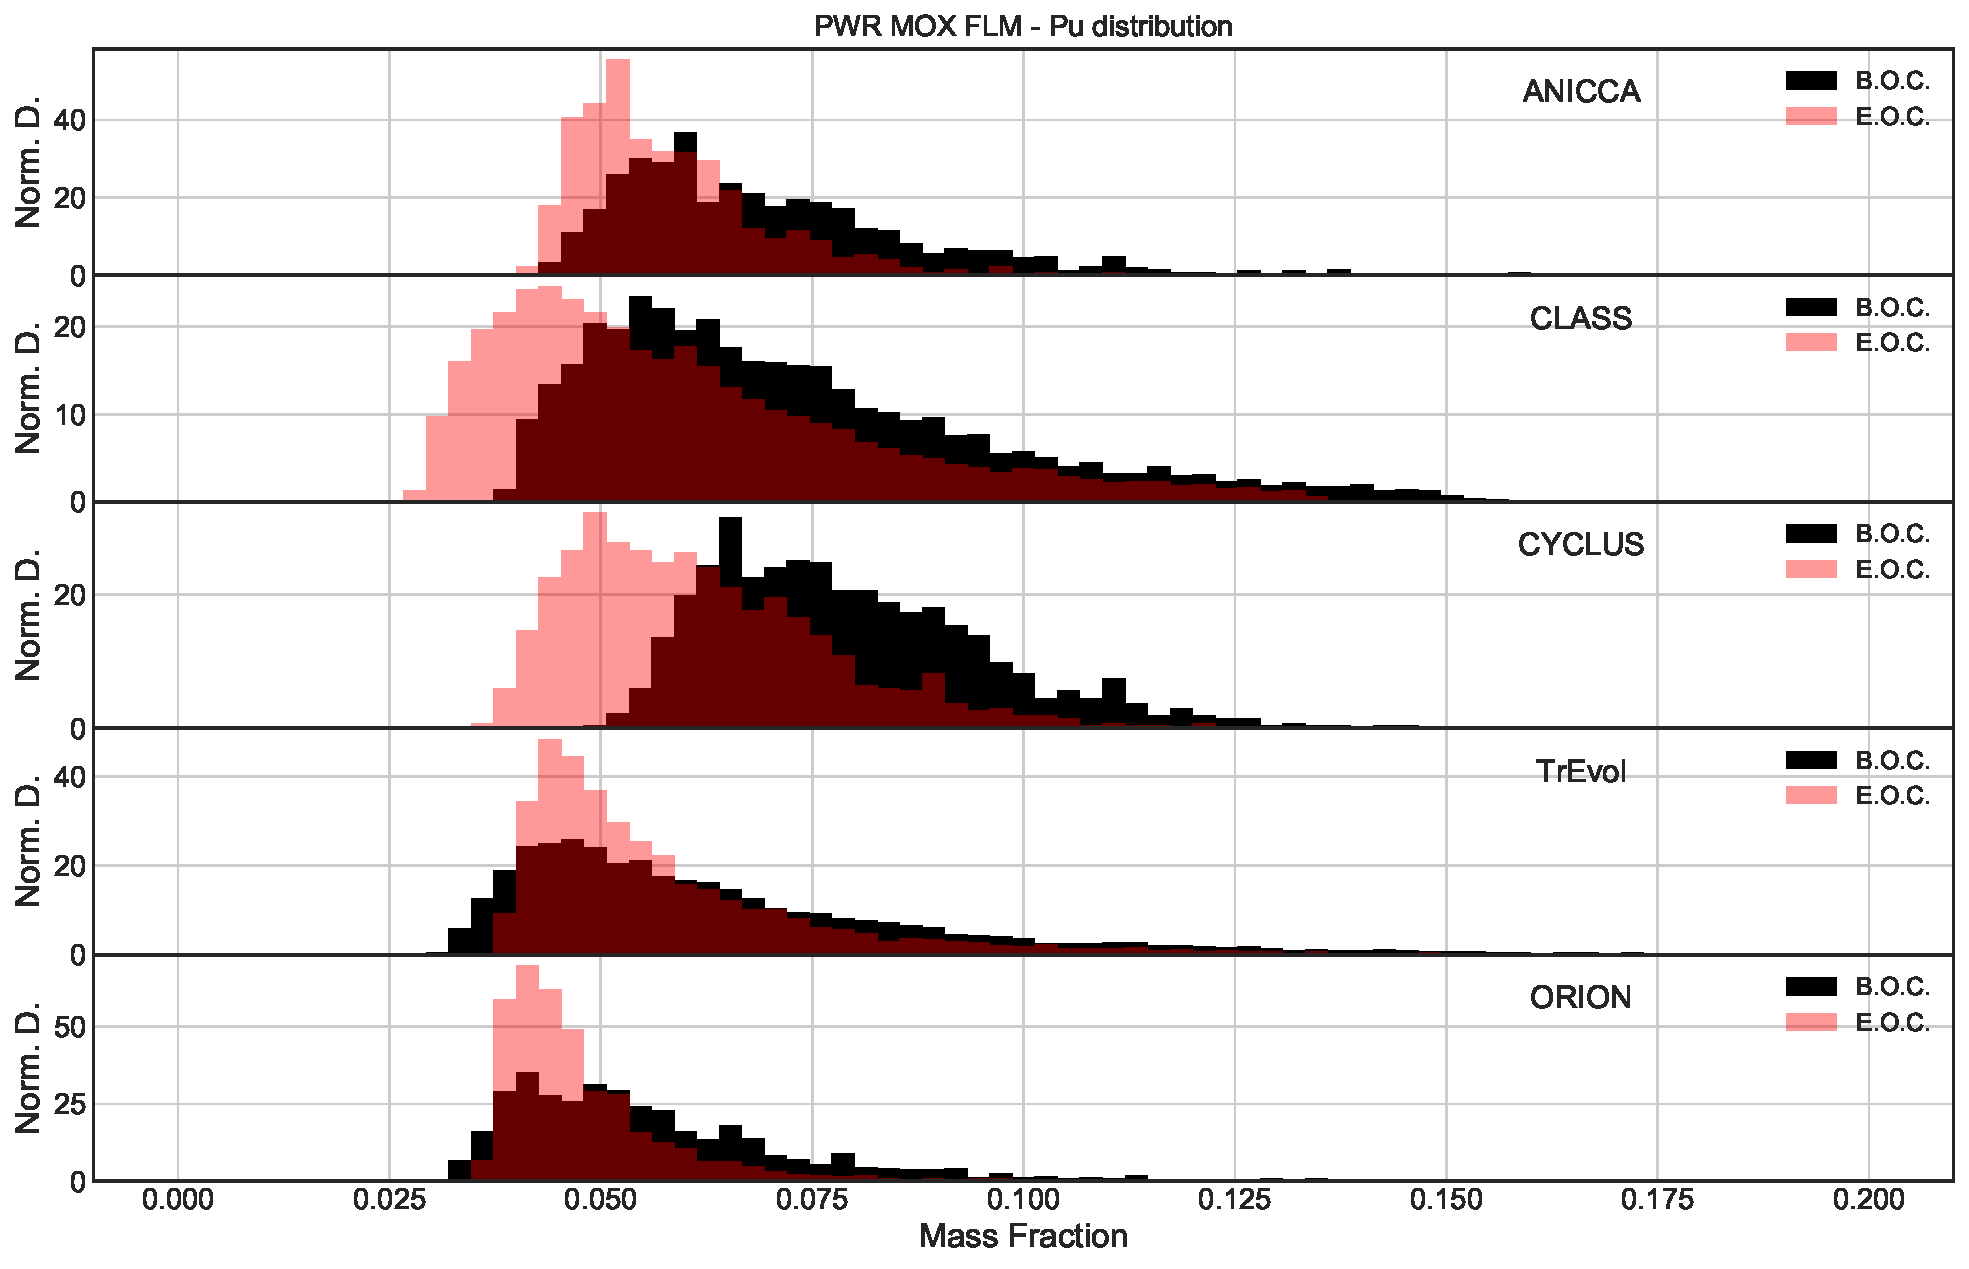
\includegraphics[width = 0.99\textwidth]{../../Feature_1/RAW_DATA/FIG/PWR_MOX_FLM_Pu.pdf}
		\caption{Code outputs for \gls{PWR} scenario's calculations}
		\label{fig:PWR_MOX_FLM_Pu}
	\end{center}
\end{figure}

The \gls{EOC} plutonium fraction is clearly shifted to the lower values, proving that
plutonium is consumed during irradiation like it should be in \gls{PWR}s. For ANICCA
and for TR\_EVOL however, some calculations show configurations where the
plutonium fraction is higher at \gls{EOC} than it is at \gls{BOC}. This unrealistic
result may be explained by the very wide plutonium isotopic composition range.
ANICCA and TR\_EVOL were not conceived to simulate evolutions of such a wide range
of compositions. This strange behavior may be attributed to the depletion
calculation of those extreme fuels. Results about estimator 2 and 3 evaluating
plutonium consumption should then be handled carefully with TR\_EVOL and ANICCA
results.   


\subsubsection{Estimator's calculation}

Figure~\ref{fig:Est1_PWR}, figure~\ref{fig:Est2_PWR} and
figure~\ref{fig:Est3_PWR} represent, for the \gls{PWR}, the distribution of the
different estimators defined in the section\ref{subsec:estimator}. 

\paragraph{Plutonium fraction at \gls{BOC}}

Estimator 1 aims to quantify bias introduced by the use of a \gls{FF} model on
the plutonium enrichment calculation for fresh fuel. It measures the amount of
plutonium used for \gls{MOX} fuel fabrication. An important positive bias means
that the \gls{FF} model estimate a lower spent fuel mass to be processed for
the MOX fuel fabrication. As the \gls{FF} was tuned on a standard plutonium
composition, in the middle of the isotopic space used for sampling,
Figure~\ref{fig:Est1_PWR} presents some histograms almost centered on 0.
        

\begin{figure}[h]
	\begin{center}
		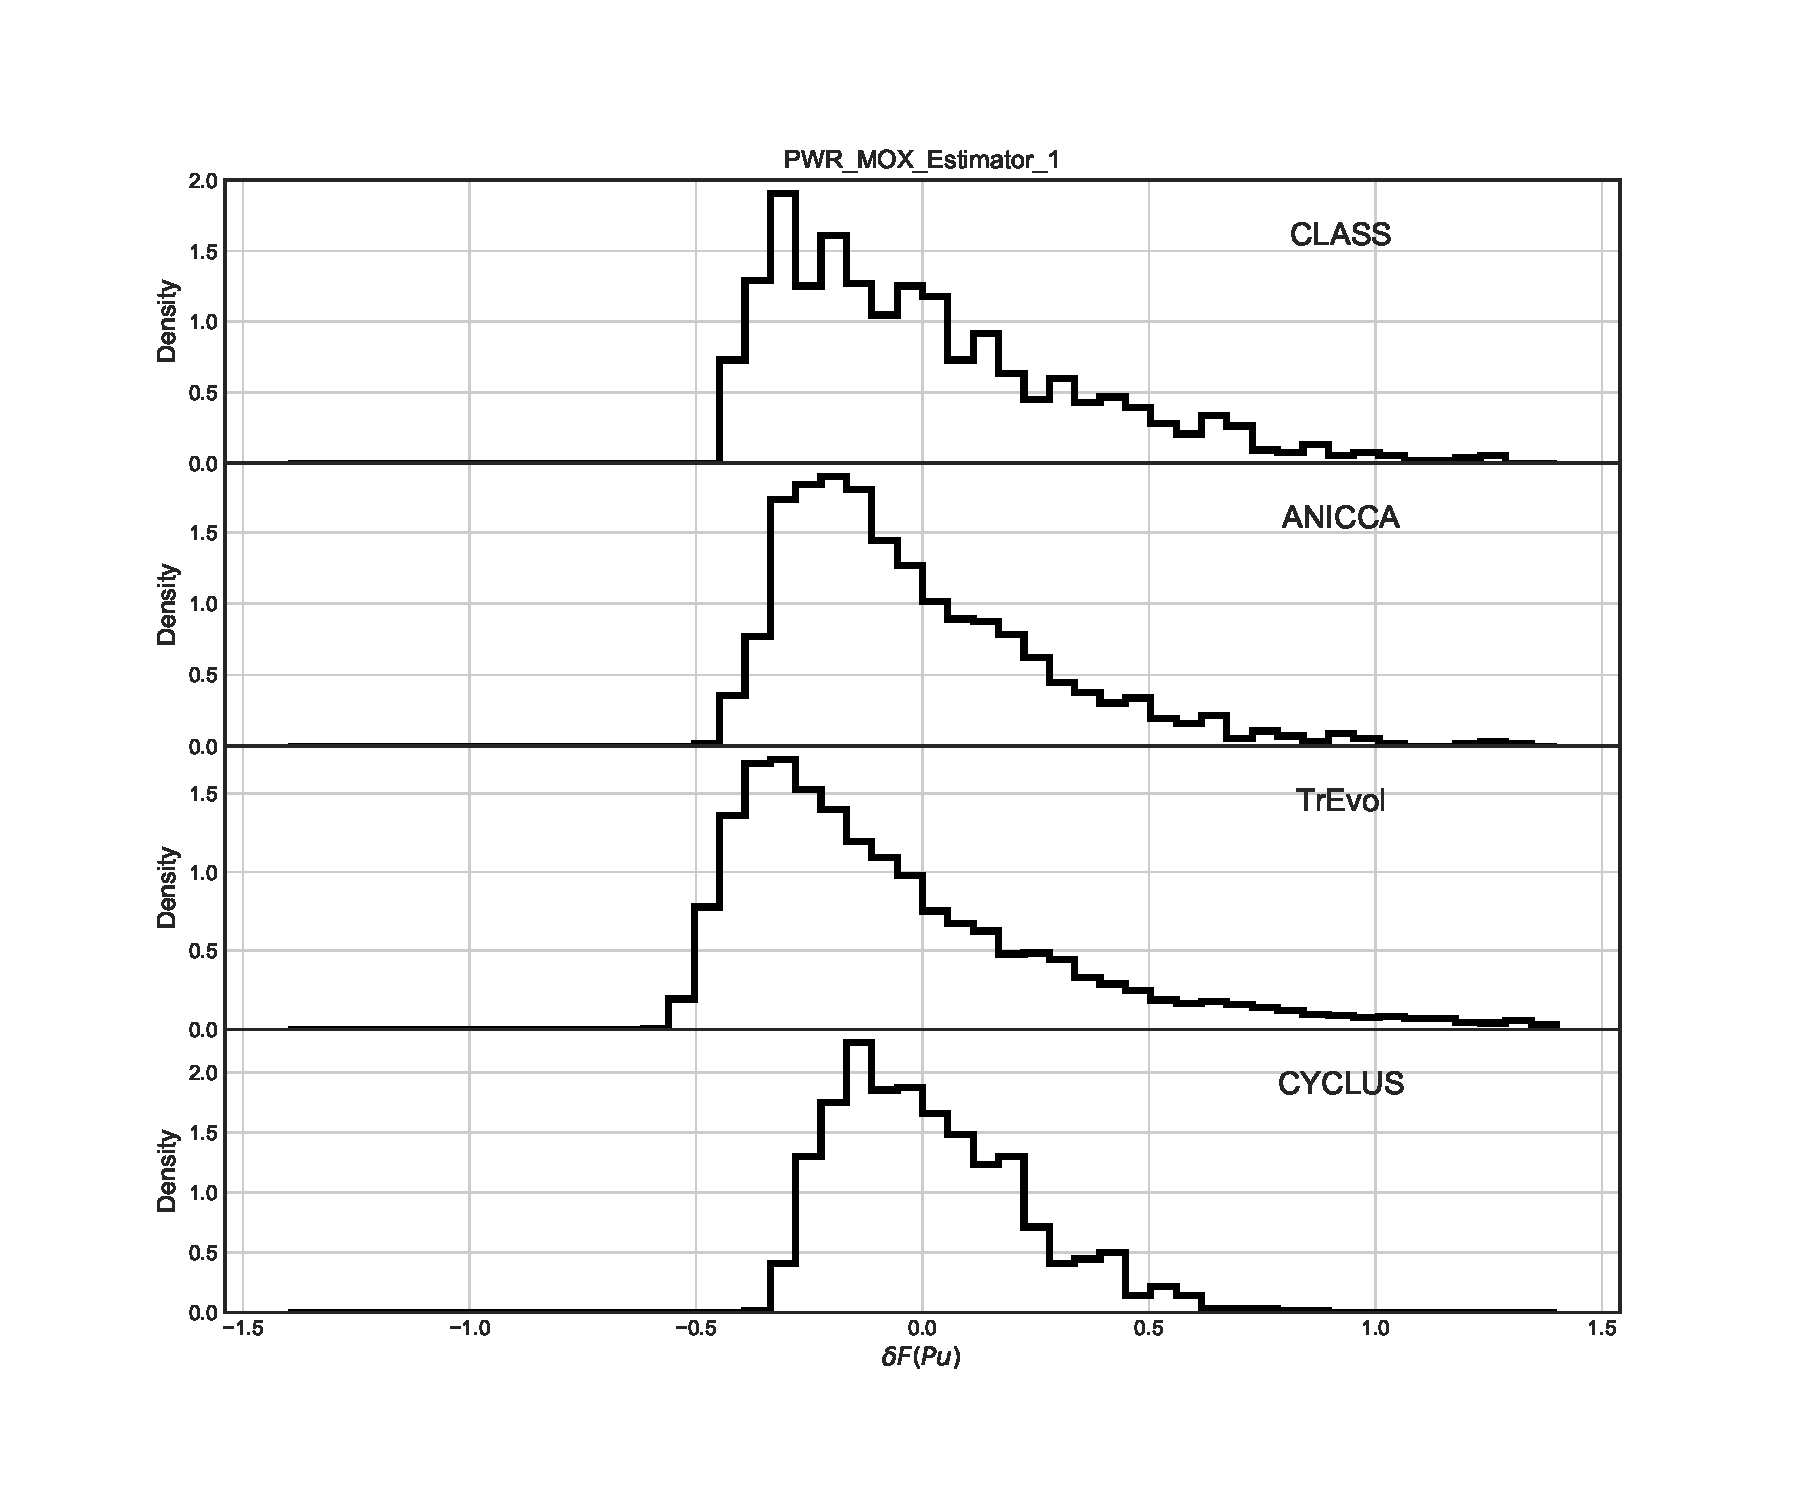
\includegraphics[width = 0.99\textwidth]{../../Feature_1/RAW_DATA/FIG/PWR_MOX_Estimator_1.pdf}
		\caption{Estimator 1 for \gls{PWR} calculated with ANICCA, CLASS, CYCLUS and TR\_EVOL}
		\label{fig:Est1_PWR}
	\end{center}
\end{figure}

The standard deviation of the distribution is also a relevant quantity as it
quantifies the dispersion of the calculation bias (i.e. i\textit{estimator 1}).
They are presented in table~\ref{table:Est1_PWR}. A small standard deviation
implies a narrow distribution and means small calculation biases due to the use
of \gls{FF} model. As we can see on the plot, none of the used software for this
work shows a small standard deviation. Meaning that, within the range of the
sampled plutonium composition, the use of a \gls{FF} model induce ``large'' bias
on the fresh \gls{MOX} fuel plutonium fraction, leading to ``large`` bias on the
mass of reprocessed spent fuel for the \gls{MOX} fuel fabrication.

\begin{table}[h]
	\begin{center}
		\begin{tabular}{|c||c||c||c|}
			\hline 
				ANICCA & CLASS & TR\_EVOL & CYCLUS \\
			\hline
				28\% & 33\% & 41\% & 20\% \\
			\hline
		\end{tabular}
	\end{center}
	\label{table:Est1_PWR}
\end{table}

\paragraph{Ratio between plutonium consumption and plutonium at \gls{BOC}}

Estimator 2 aims to quantify the amount of plutonium consumption regarding the
plutonium mass at \gls{BOC}. It measures the proportion of plutonium burnt
during irradiation. Estimator 2 distribution gives an evaluation of the total
inventory precision estimation, regardless the location of the plutonium.
Figure~\ref{fig:Est2_PWR} represents the different distributions of this estimator
for the 4 codes used in this part. There are two trends in this plot: CYCLUS and
CLASS shows limited bias (with a standard deviation of 12\% and 8\% respectively as it
can be seen in table~\ref{table:Est2_PWR}), whereas TR\_EVOL and ANICCA
calculates very strong biases. From this different behaviors, it is impossible
to conclude on the \gls{FLM} relevance for total inventory estimation. A limited bias
(as seen with CYCLUS and CLASS) means that the use of a \gls{FF} for plutonium
enrichment at \gls{BOC} may be sufficient for global inventory estimation. On the
opposite, results from ANICCA and TR\_EVOL tends to show that a \gls{FLM} is
necessary. 

\begin{figure}[h]
	\begin{center}
		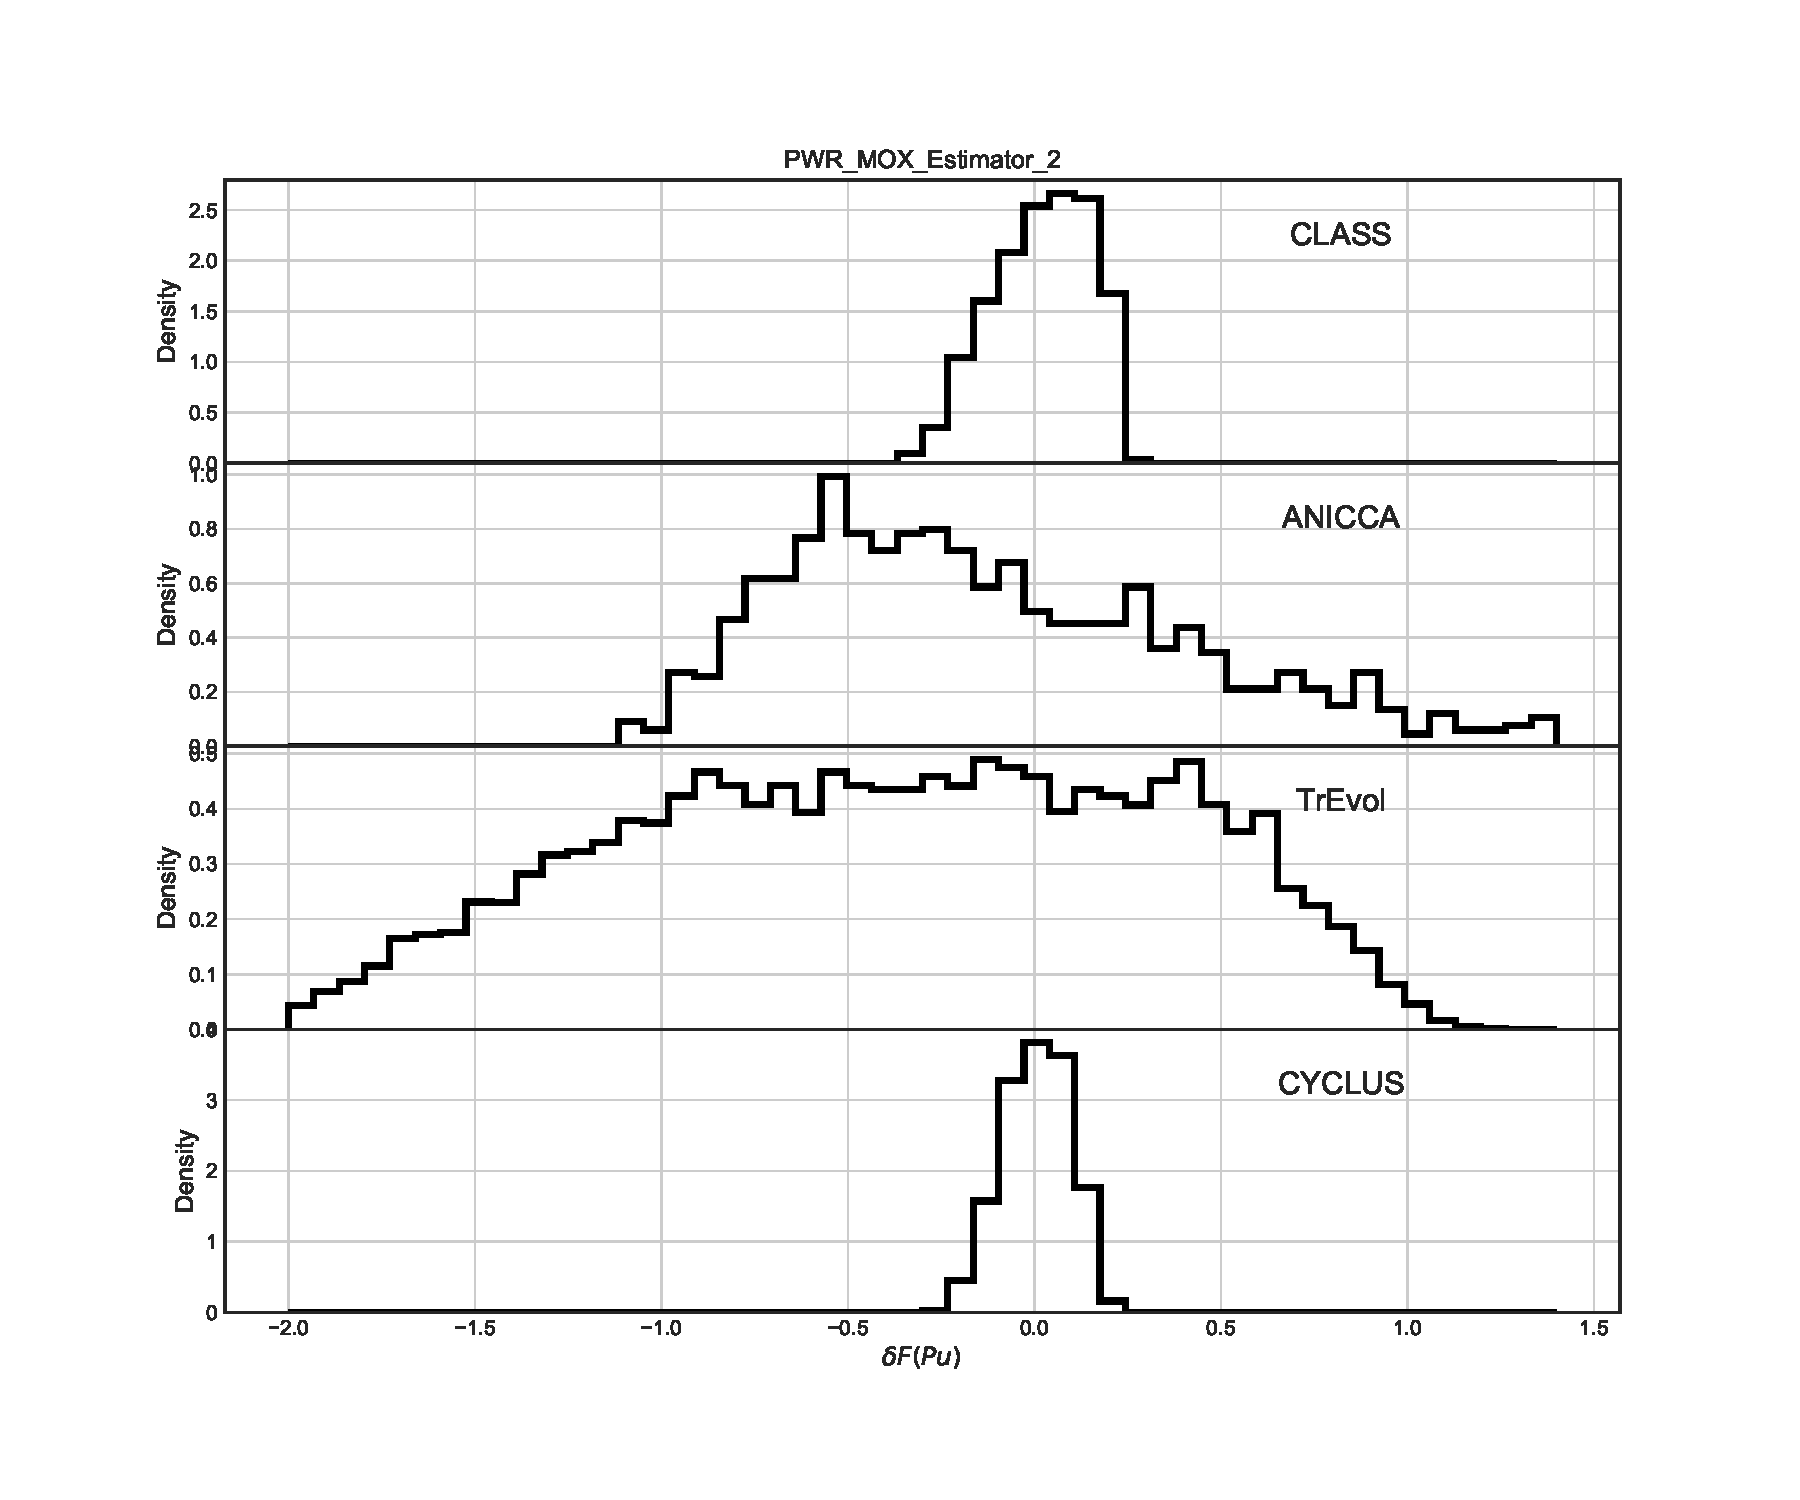
\includegraphics[width = 0.99\textwidth]{../../Feature_1/RAW_DATA/FIG/PWR_MOX_Estimator_2.pdf}
		\caption{Estimator 2 for \gls{PWR} calculated with CLASS, CYCLUS and TR\_EVOL}
		\label{fig:Est2_PWR}
	\end{center}
\end{figure}

\begin{table}[h]
	\begin{center}
		\begin{tabular}{|c||c||c||c|}
			\hline 
				ANICCA & CLASS & TR\_EVOL & CYCLUS \\
			\hline
				59\% & 12\% & 71\% & 9\% \\
			\hline
		\end{tabular}
	\end{center}
	\label{table:Est2_PWR}
\end{table}

It has to be pointed out that this estimator (as for estimator 3 shown in the
next paragraph) needs a depletion calculation.  Figure~\ref{fig:PWR_MOX_FLM_Pu}
shows that this depletion calculation is questionable for some plutonium
isotopic compositions with ANICCA and TR\_EVOL.  Those two software may be used
beyond their validity domain and this might be reflected in the very wide
distribution of Estimator 2. The depletion calculation, inaccurate for
composition outside of the validity domain, adds some biases to the one brought
by the \gls{FF} model uses. The conclusions made with ANICCA and TR\_EVOL has
then to be consider with caution.

\paragraph{Plutonium consumption rate}

Estimator 3 measures biases on the plutonium consumption rate calculation. As
so, it measures the biases induced by a \gls{FF} for plutonium enrichment at
\gls{BOC} on a global scale. It aims to quantify the global inventory evolution
rate.  Figure~\ref{fig:Est3_PWR} represents estimator 3 for CLASS, ANICCA,
TR\_EVOL and CYCLUS. Similar conclusion can be drawn as previous section. CLASS
and CYCLUS are in agreement as shows that the impact of using a \gls{FF} may be
limited, introducing between $11\%$ for CYCLUS and $18\%$ for CLASS bias on the total plutonium consumption rate. On the
contrary ANICCA and TR\_EVOL are also in agreement showing a much larger bias ($105\%$ and $108\%$ respectively).
The same caution of previous section should be pointed out: depletion
calculation of the latest software are out of validity domain adding some
uncertainty to the bias calculated by the use of \gls{FLM}.       

\begin{figure}[h]
	\begin{center}
		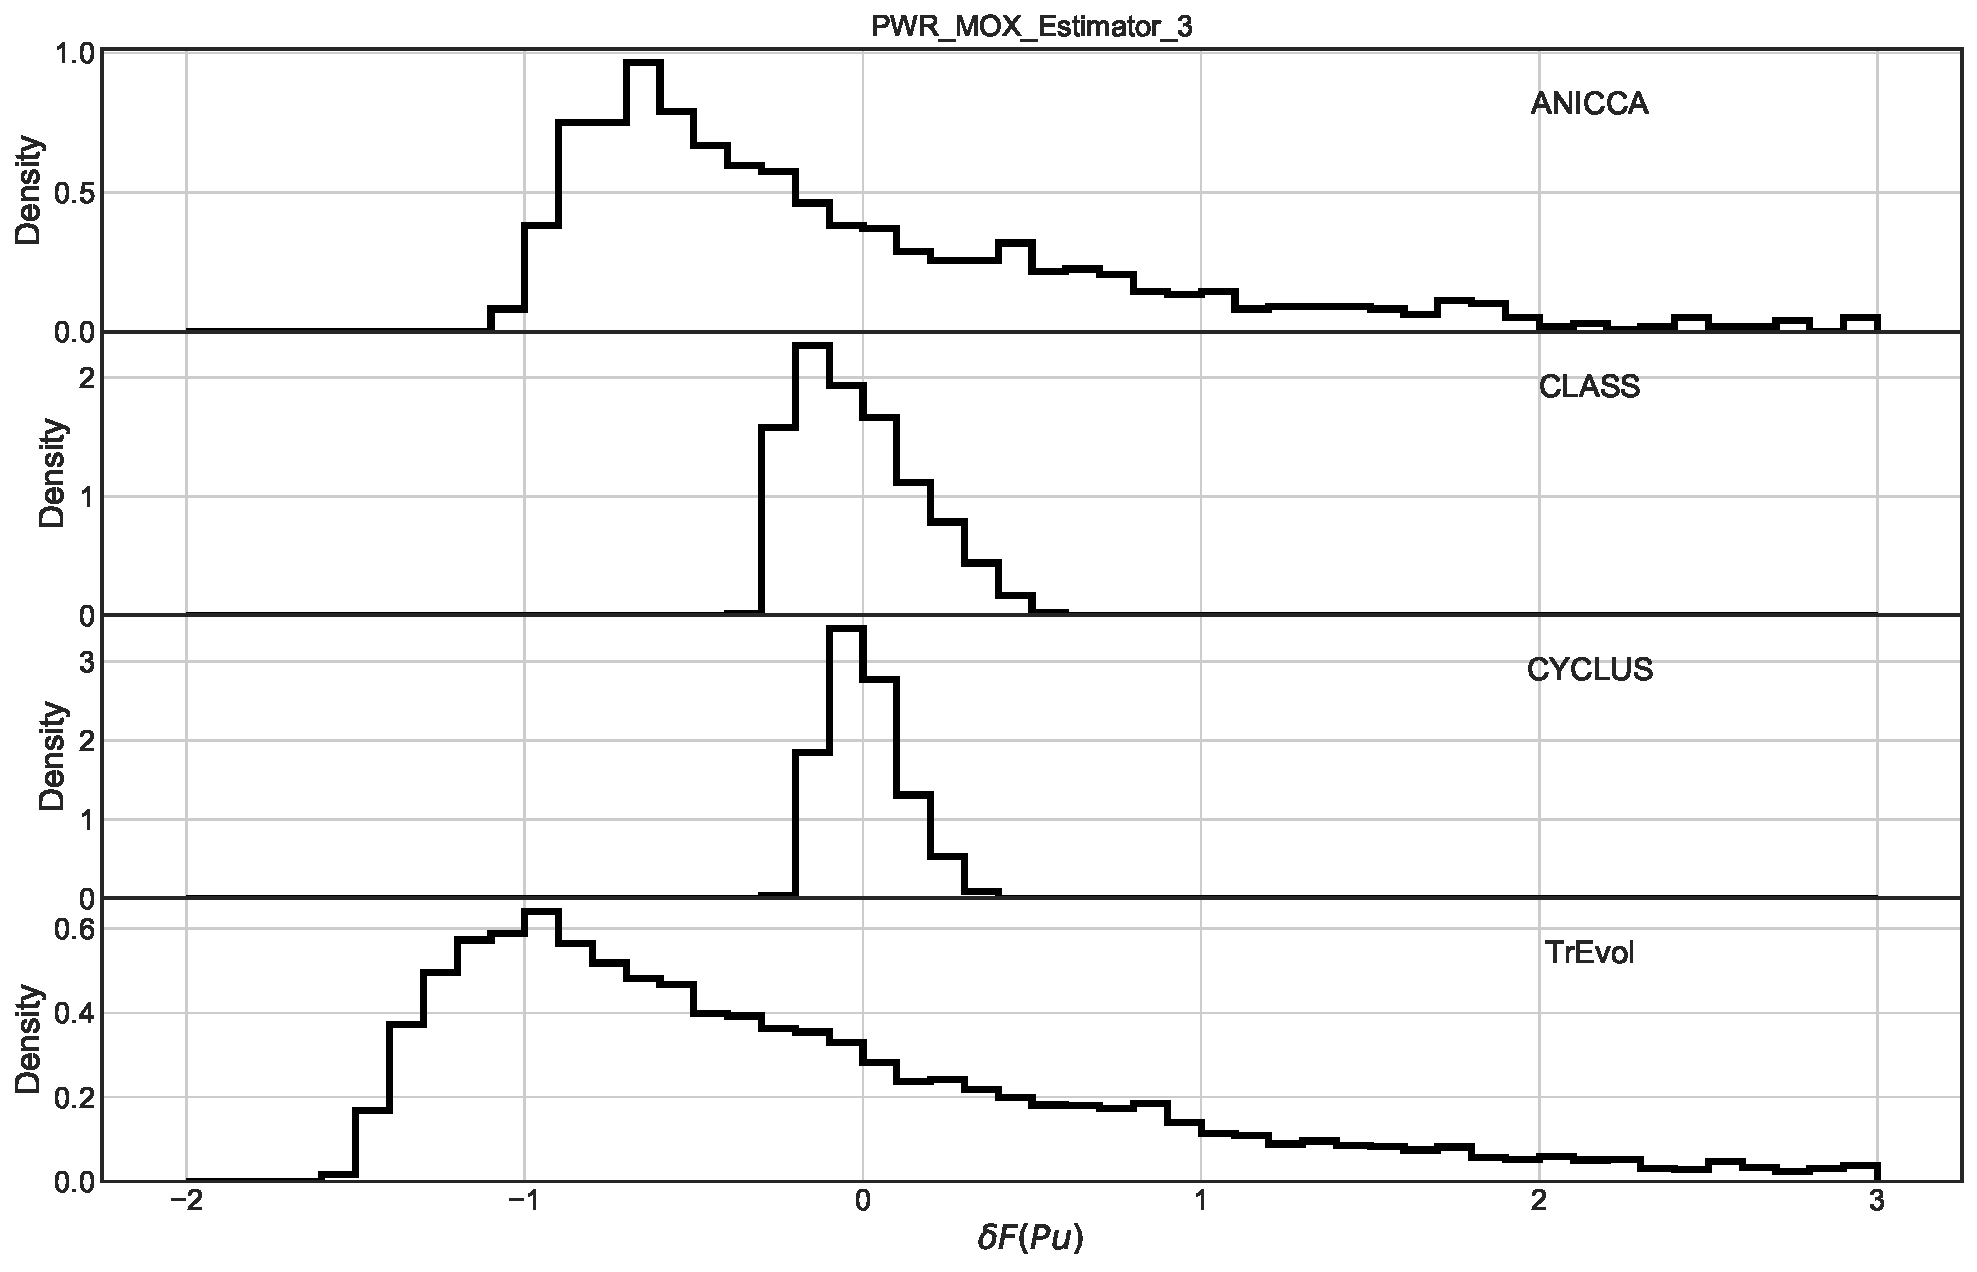
\includegraphics[width = 0.99\textwidth]{../../Feature_1/RAW_DATA/FIG/PWR_MOX_Estimator_3.pdf}
		\caption{Estimator 3 for \gls{PWR} calculated with CLASS, CYCLUS and TR\_EVOL}
		\label{fig:Est3_PWR}
	\end{center}
\end{figure}

\subsection{Fast Sodium cooled Reactor}
\subsubsection{Output analyses}

Figure~\ref{SFR_MOX_FLM_Pu} represents the plutonium enrichment distribution at
BOC (in black) and at \gls{EOC} (in red) simulated with CLASS, JOSETTE and TR\_EVOL.
The difference between reactor models used by the different software explain the
different behaviors. Indeed CLASS simulates a breeder whereas TR\_EVOL simulate a
burner and JOSETTE a break-even reactor. Plutonium mass evolution is then
different across all those software. The purpose of this work is not to compare
software but to compare the use or not of the \gls{FLM}. The reactor models
showing different behavior reinforces conclusions drawn for the importance of
\gls{FLM} in fuel cycle simulators.     

\begin{figure}[h]
	\begin{center}
		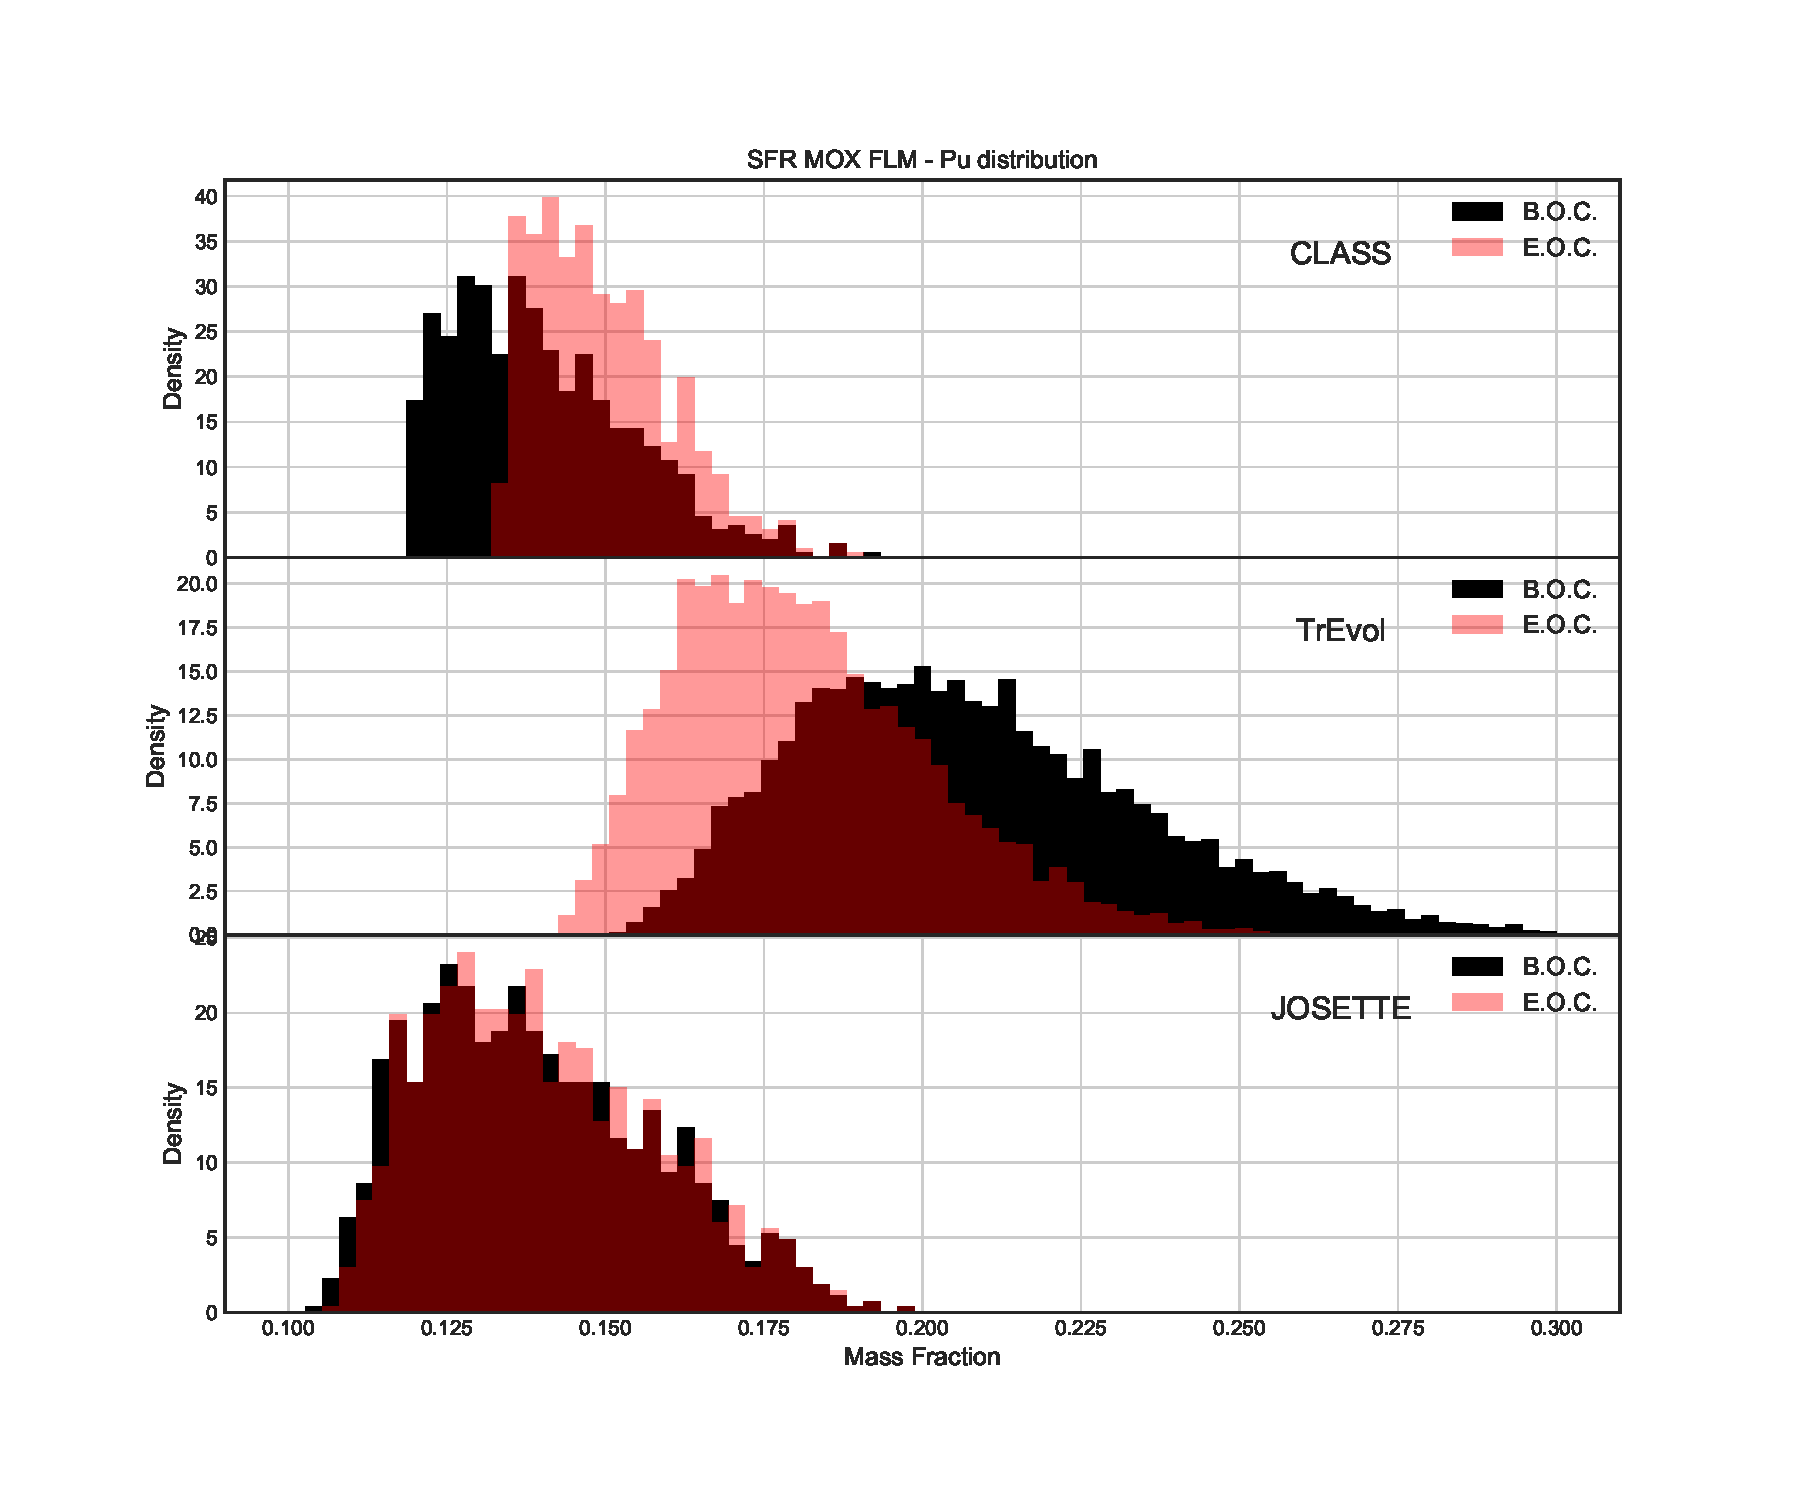
\includegraphics[width = 0.99\textwidth]{../../Feature_1/RAW_DATA/FIG/SFR_MOX_FLM_Pu.pdf}
		\caption{Code outputs for \gls{PWR} scenario's calculations}
		\label{fig:SFR_MOX_FLM_Pu}
	\end{center}
\end{figure}

\subsubsection{Estimator's calculation}
\paragraph{Plutonium fraction at \gls{BOC}}

Figure~\ref{fig:Est1_SFR} represents the estimator 1 calculated for Sodium
Cooled Fast Reactors calculated with JOSETTE, TR\_EVOL and CLASS. As for
\gls{PWR}, it shows the relative difference of plutonium enrichment with the use
of a \gls{FLM} with regards to a \gls{FF}. Standard deviations of the difference
distribution is given in Table~\ref{table:Est1Dev_SFR} for the different
simulators. All of them are in agreement even if CLASS slightly estimate a
smaller \gls{FF} impact on the plutonium needed for a \gls{SFR}. The typical bias
produced by the use of a \gls{FF} is smaller than 25\% and is much lower than
for \gls{PWR}.   

\begin{figure}[h]
	\begin{center}
		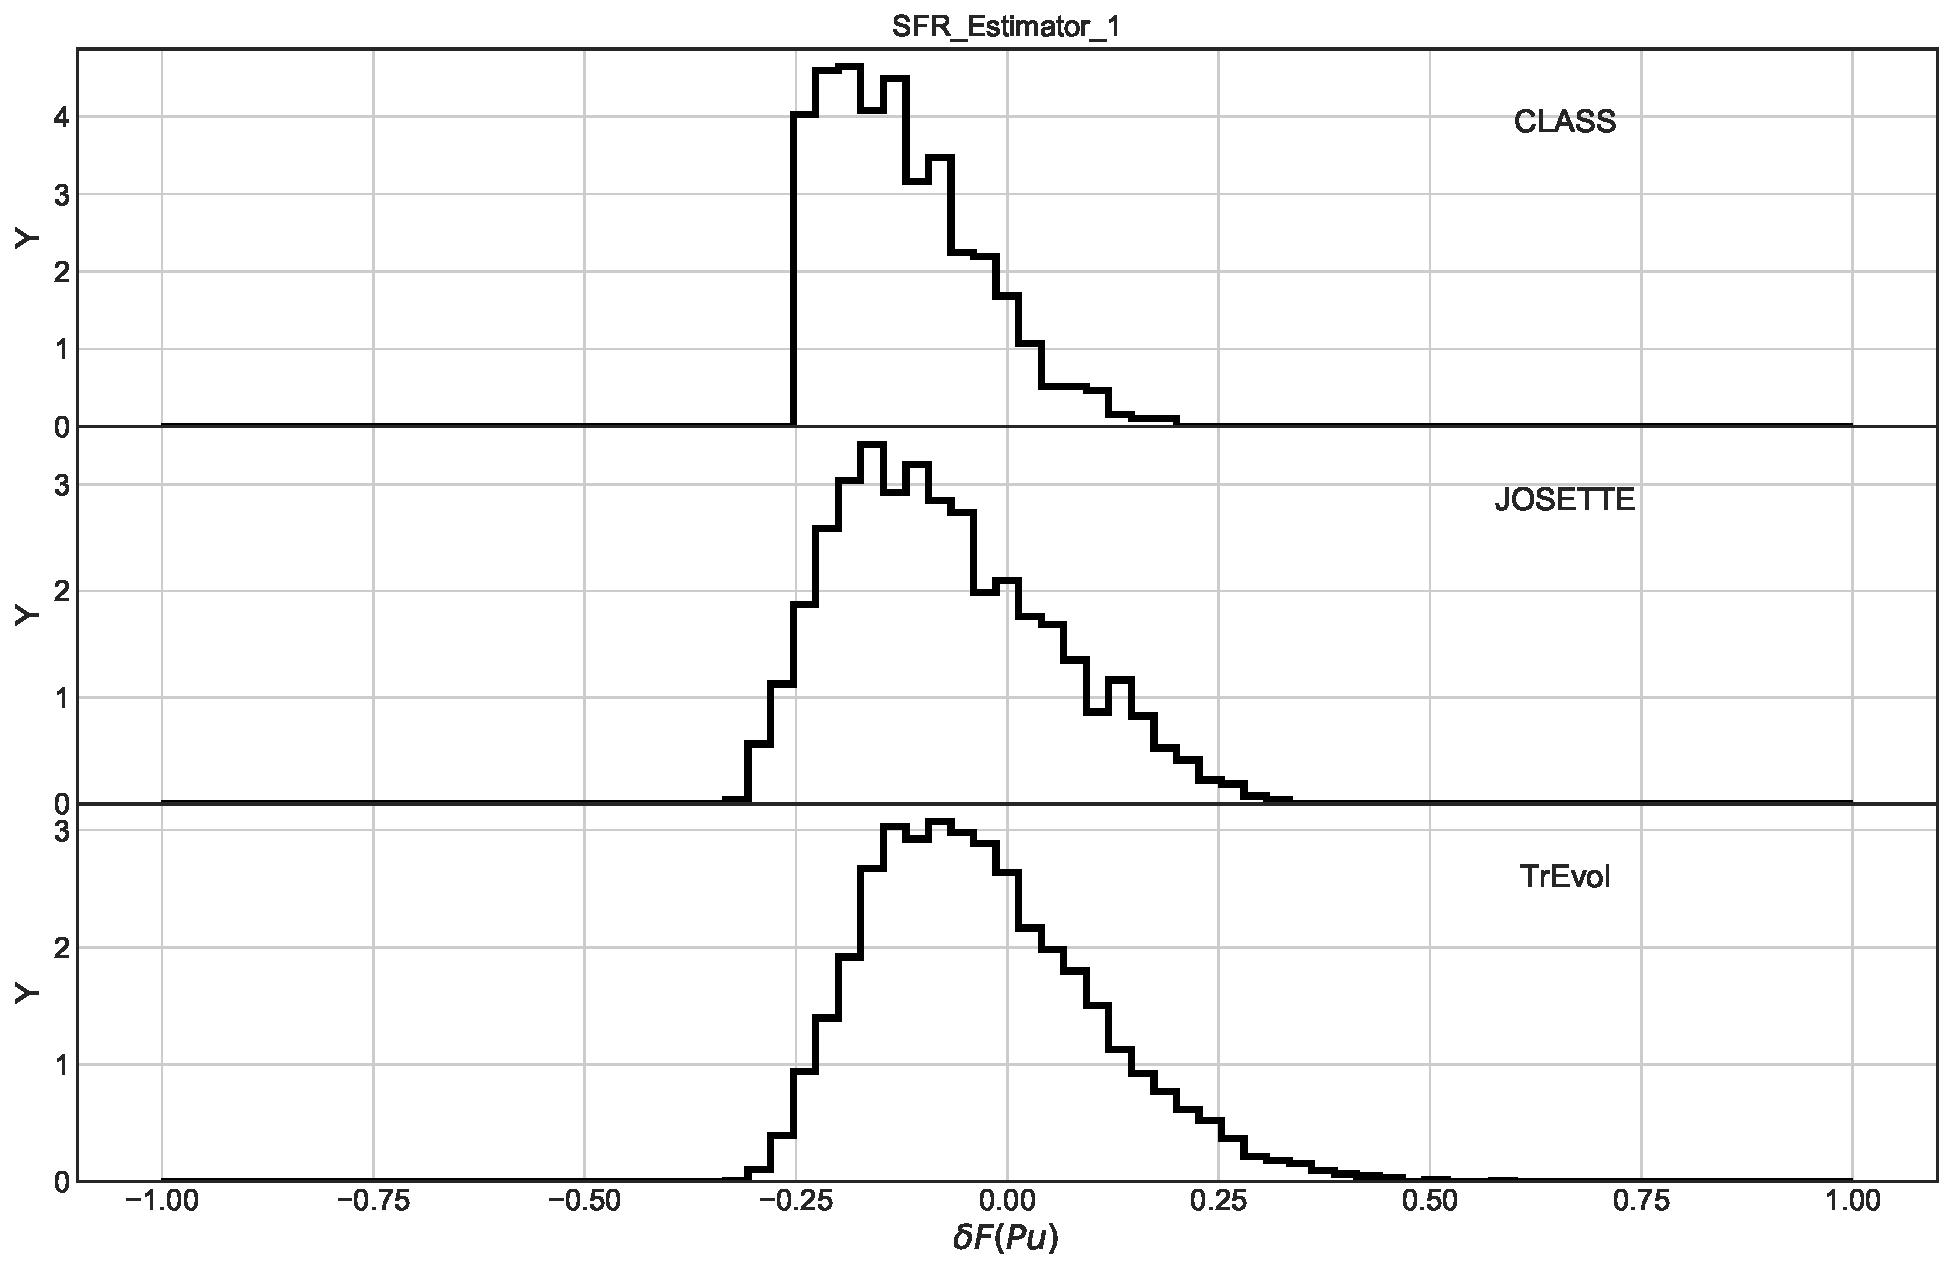
\includegraphics[width = 0.99\textwidth]{../../Feature_1/RAW_DATA/FIG/SFR_Estimator_1.pdf}
		\caption{Estimator 1 for \gls{SFR} calculated with JOSETTE, TR\_EVOL, and CLASS}
		\label{fig:Est1_SFR}
	\end{center}
\end{figure}

\begin{table}[h]
	\begin{center}
		\begin{tabular}{|c||c||c|}
			\hline 
				CLASS & JOSETTE & TR\_EVOL \\
			\hline
				9\% & 12\% & 13\% \\
			\hline
		\end{tabular}
	\end{center}
	\label{table:Est1Dev_SFR}
\end{table}

The spent fuel mass to be reprocessed for \gls{SFR} fresh fuel using a \gls{FF}
for plutonium enrichment is then estimated with a bias smaller than 10\%
regardless of the \gls{SFR} behavior (breeder, burner or break-even).  

\paragraph{Ratio between plutonium consumption and plutonium at \gls{BOC}}

Estimator 2.b aims to calculate the plutonium production or consumption at the
simulation global level. It estimates the absolute difference on breeding
ratio between a \gls{FF} and a \gls{FLM}. CLASS and TR\_EVOL show similar
results. Both calculate biases induced by the \gls{FF} up to 0.1. JOSETTE
calculations shows a narrower distribution, probably due to a
break-even simulated \gls{SFR}.   

\begin{figure}[h]
	\begin{center}
		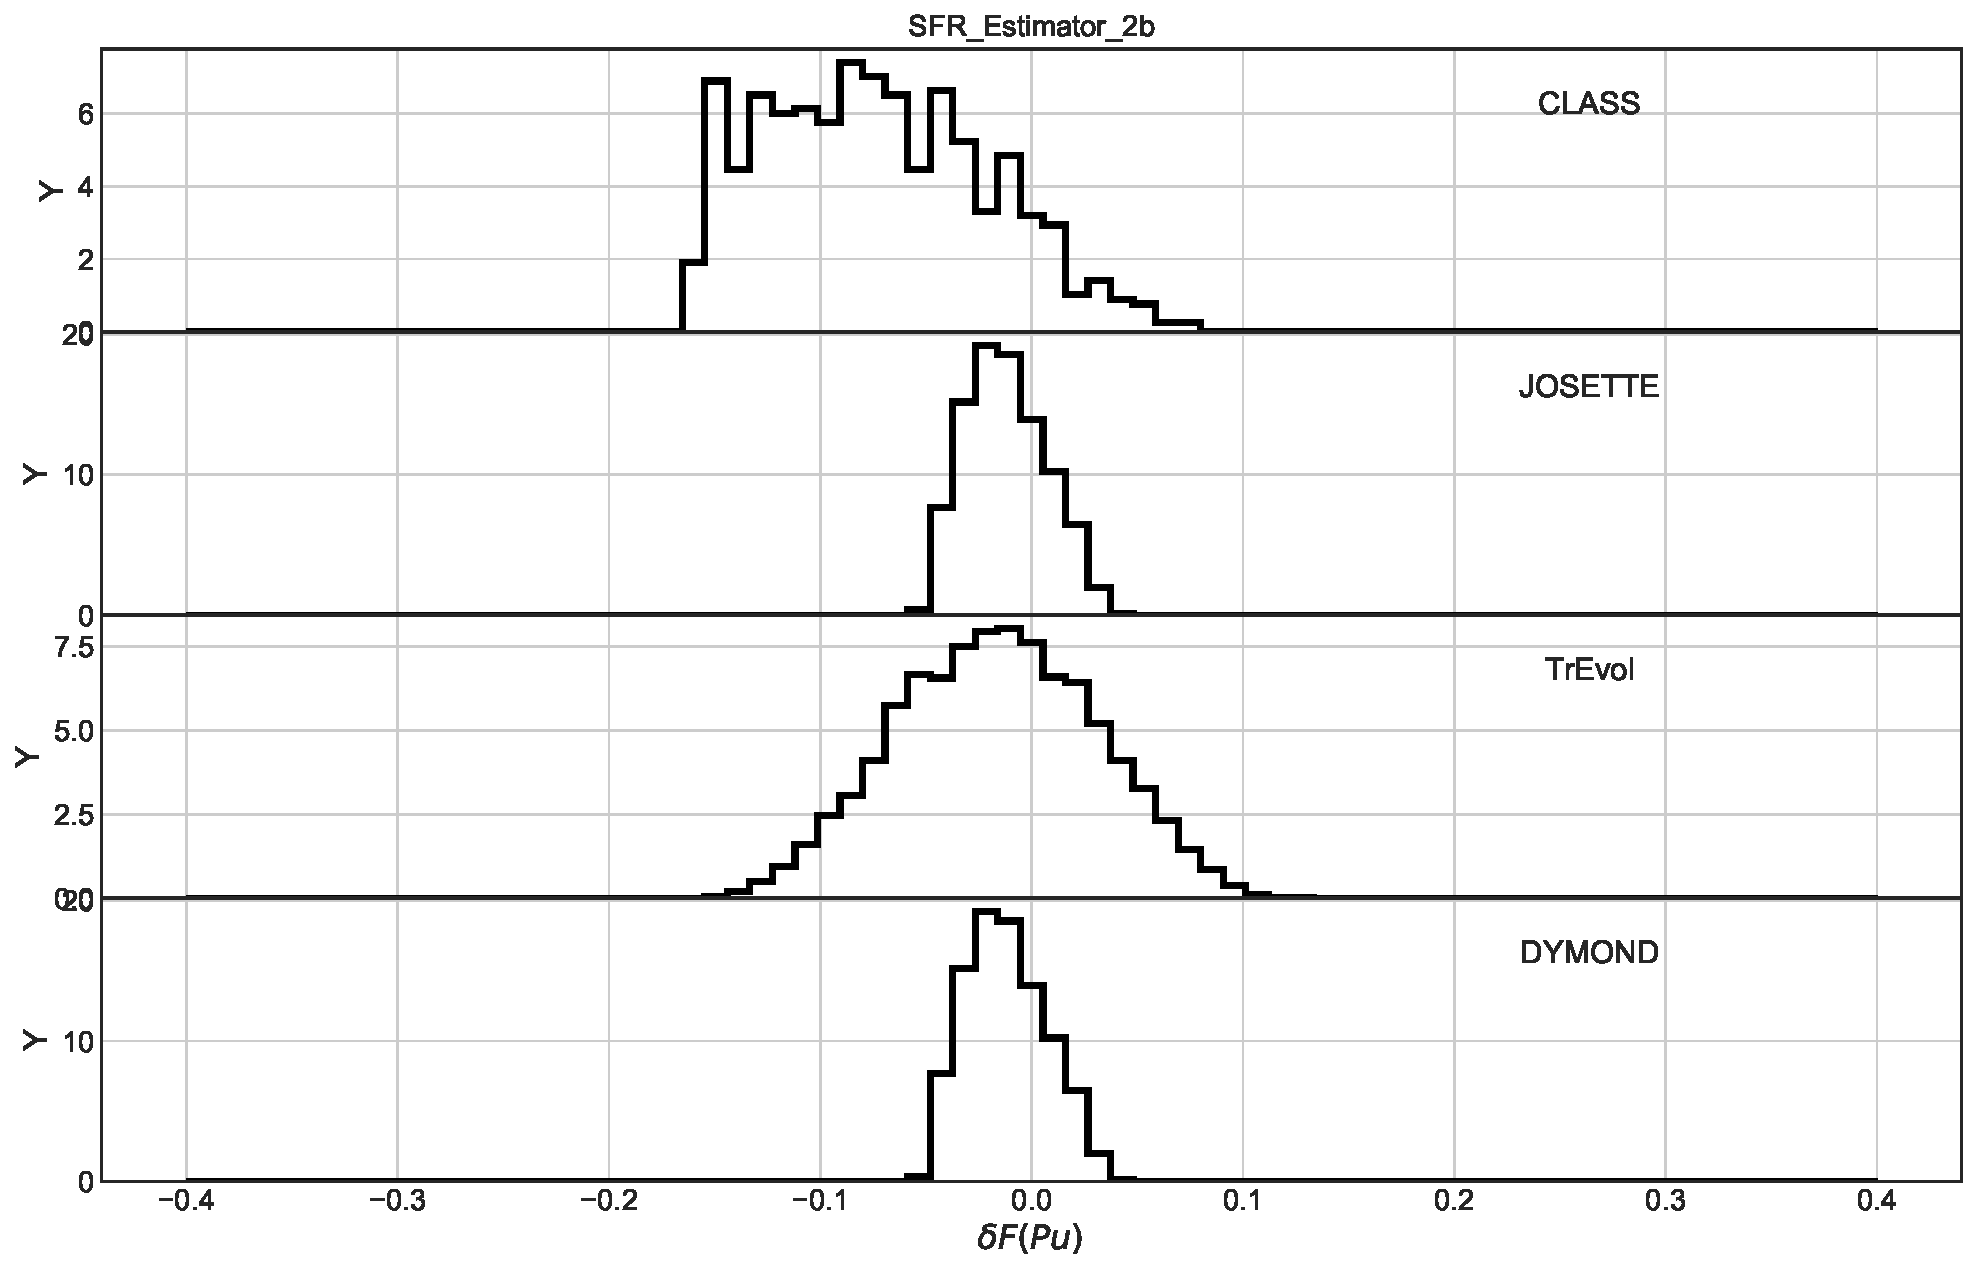
\includegraphics[width = 0.99\textwidth]{../../Feature_1/RAW_DATA/FIG/SFR_Estimator_2b.pdf}
		\caption{Estimator 2.b for \gls{SFR} calculated with JOSETTE, TR\_EVOL, and CLASS}
		\label{fig:Est2_SFR}
	\end{center}
\end{figure}
